\documentclass{beamer}

\usepackage{mpemath}
\usepackage{subcaption}
\usepackage[normalem]{ulem}
\usepackage{amsmath}
\usepackage{amssymb}
\usepackage{mathtools}
\usepackage{booktabs}
\usepackage{siunitx}
\usepackage{natbib}
\usepackage{tabularx}
\usepackage{multirow}
\usepackage{amsmath}
\usepackage{mathtools}
\usepackage{amssymb}
\usepackage{bbm}
\usepackage[dvipsnames]{xcolor} % Saved my life during a conference once

% *** Styles ***
\usetheme{Singapore}
\setbeamertemplate{navigation symbols}{}
\setbeamercovered{invisible}
\usefonttheme{professionalfonts}
\setbeamertemplate{footline}[frame number]

\title{PPO Workshop}
\author{Gersi Doko}
\institute{Department of Computer Science \\ University of New Hampshire}
\date{}

\AtBeginSection[]{
  \begin{frame}
    \vfill
    \centering
    % \usebeamerfont{title}
    {\huge\bf \insertsectionhead}%
    \vfill
  \end{frame}
}

\begin{document}

\frame{\titlepage}

\section*{Intro}

\begin{frame}
  \frametitle{What is PPO?}
  \vfill
  \begin{enumerate}
    \item PPO is REINFORCE with `clipping'
    \item We will only think in terms of \emph{inputs} and \emph{outputs}
  \end{enumerate}
\end{frame}

\begin{frame}
  \frametitle{Preliminaries}
  $\pi_\theta(a | s)$ - policy parameterized by $\theta$\\
  \vfill
  $V^{\pi_\theta}(s)$ - value function of $\pi_\theta$\\
  \vfill
  $L(\theta)$ - loss function to be optimized
\end{frame}

\begin{frame}
  \frametitle{Preliminaries - Inputs and Outputs}
  $\pi_\theta(a | s)$ - make decisions about what action to take
  given the state it is in and the parameters $\theta$\\
  \vfill
  $V^{\pi_\theta}(s)$ - estimate of future discounted rewards given
  the state it is in and the policy $\pi_\theta$\\
  \vfill
  $L(\theta)$ - a number that we want to minimize by changing
  $\theta$, the lower the number the better the model is doing
\end{frame}

\section*{PPO}

\begin{frame}
  \frametitle{As easy as 1, 2, 3}
  \vfill
  \begin{figure}[ht]
    \centering
    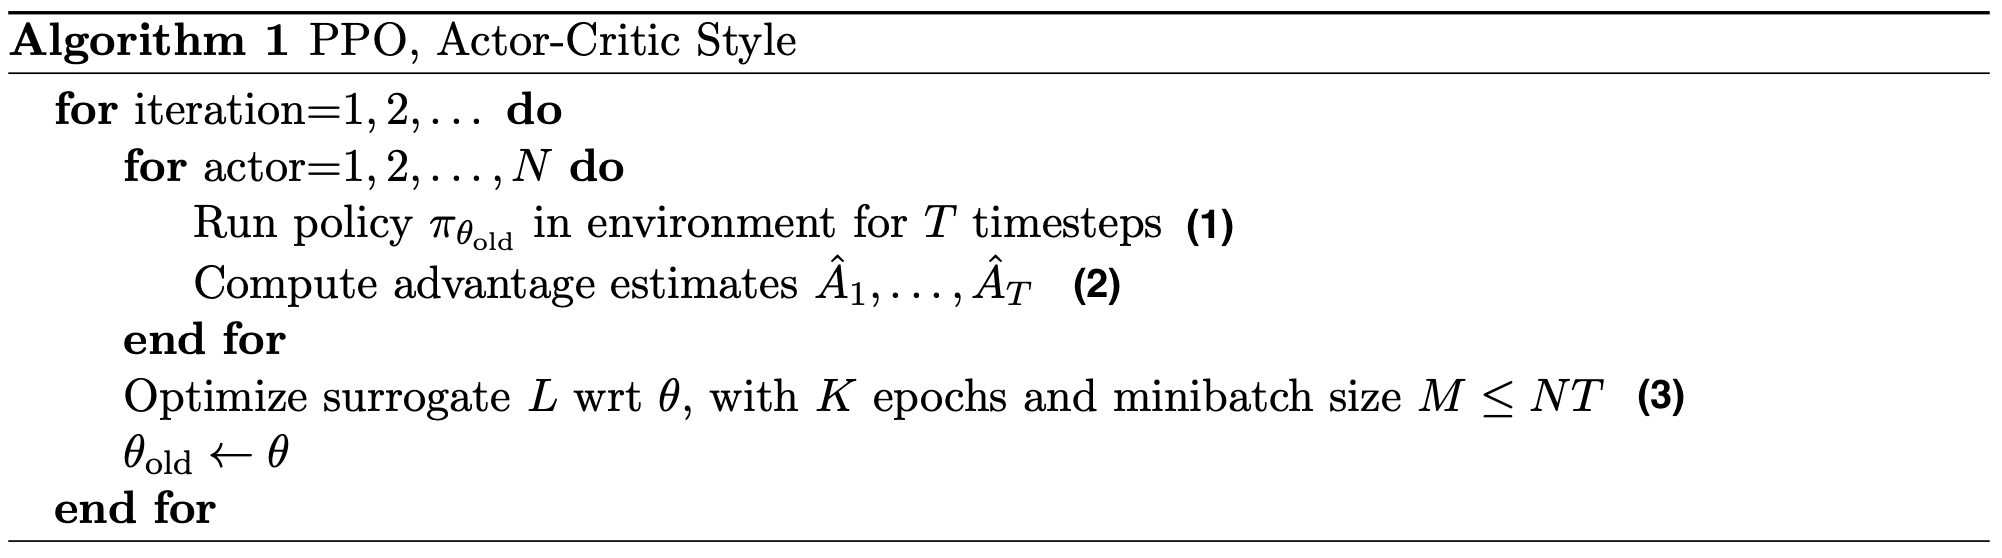
\includegraphics[width=\textwidth]{./imgs/1.png}
  \end{figure}
  \vfill
\end{frame}

\begin{frame}
  \frametitle{As easy as 1, 2, 3}
  \vfill
  \begin{figure}[ht]
    \centering
    
\includegraphics[width=\textwidth]{./imgs/2.png}
  \end{figure}
  \vfill
\end{frame}

\begin{frame}
  \frametitle{As easy as 1, 2, 3}
  \vfill
  \begin{figure}[ht]
    \centering
    
\includegraphics[width=\textwidth]{./imgs/2.png}
  \end{figure}
  \vfill
  \begin{enumerate}
    \item What are the inputs?
    \item What are the outputs?
  \end{enumerate}
\end{frame}

\begin{frame}
  \frametitle{As easy as 1, 2, 3}
  \vfill
  \begin{figure}[ht]
    \centering
    
\includegraphics[width=\textwidth]{./imgs/2.png}
  \end{figure}
  \vfill
  \begin{enumerate}
    \item What are the inputs? - $\pi_\theta$, $\pi_{\theta_{old}}$
    \item What are the outputs? - $(s_t, a_t, r_t, s_{t+1})_{t=0}^T \sim
      \pi_{\theta_{old}}$
  \end{enumerate}
\end{frame}

\begin{frame}
  \frametitle{As easy as 1, 2, 3}
  \vfill
  \begin{figure}[ht]
    \centering
    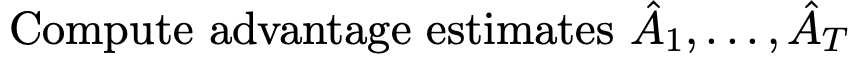
\includegraphics[width=\textwidth]{./imgs/3.png}
  \end{figure}
  \vfill
\end{frame}

\begin{frame}
  \frametitle{As easy as 1, 2, 3}
  \vfill
  \begin{figure}[ht]
    \centering
    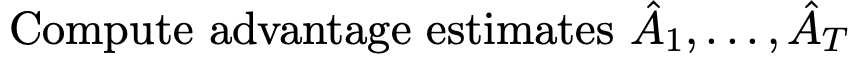
\includegraphics[width=\textwidth]{./imgs/3.png}
    \vfill
    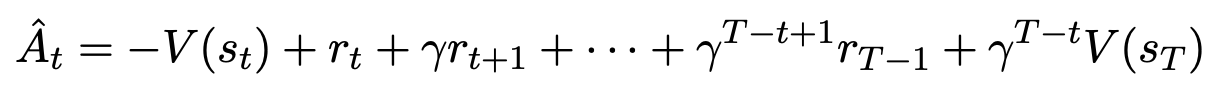
\includegraphics[width=\textwidth]{./imgs/advantages.png}
  \end{figure}
  \vfill
\end{frame}

\begin{frame}
  \frametitle{As easy as 1, 2, 3}
  \vfill
  \begin{figure}[ht]
    \centering
    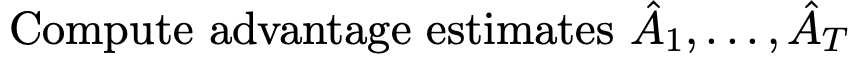
\includegraphics[width=\textwidth]{./imgs/3.png}
    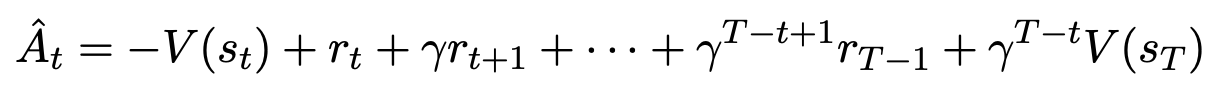
\includegraphics[width=\textwidth]{./imgs/advantages.png}
  \end{figure}
  $\hat{A}_t = \sum_{t=0}^T \gamma^t r_t - V(s_t)$
\end{frame}

\begin{frame}
  \frametitle{As easy as 1, 2, 3}
  \vfill
  \begin{figure}[ht]
    \centering
    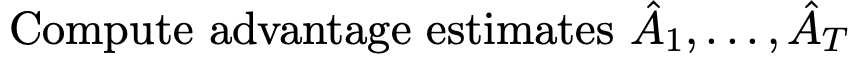
\includegraphics[width=\textwidth]{./imgs/3.png}
    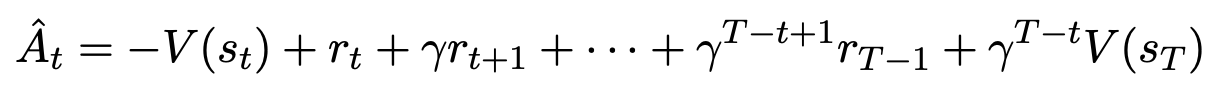
\includegraphics[width=\textwidth]{./imgs/advantages.png}
  \end{figure}
  $\hat{A}_t = \sum_{t=0}^T \gamma^t r_t - V(s_t)$
  \vfill
  \begin{enumerate}
    \item What are the inputs?
    \item What are the outputs?
  \end{enumerate}
\end{frame}

\begin{frame}
  \frametitle{As easy as 1, 2, 3}
  \vfill
  \begin{figure}[ht]
    \centering
    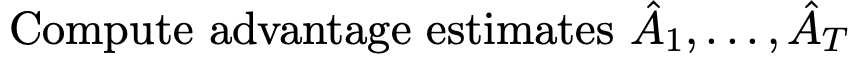
\includegraphics[width=\textwidth]{./imgs/3.png}
    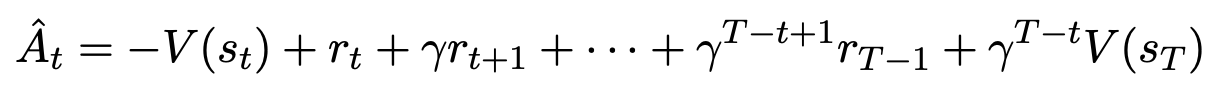
\includegraphics[width=\textwidth]{./imgs/advantages.png}
  \end{figure}
  $\hat{A}_t = \sum_{t=0}^T \gamma^t r_t - V(s_t)$
  \vfill
  \begin{enumerate}
    \item What are the inputs? - $(s_t, a_t, r_t, s_{t+1})_{t=0}^T \sim
      \pi_{\theta_{old}}$, $V^{\pi_{\theta_{old}}}(s_t)$
    \item What are the outputs? - $(\hat{A}_t)_{t=0}^T$
  \end{enumerate}
\end{frame}

\begin{frame}
  \frametitle{As easy as 1, 2, 3}
  \vfill
  \begin{figure}[ht]
    \centering
    
\includegraphics[width=\textwidth]{./imgs/4.png}
    \vfill
    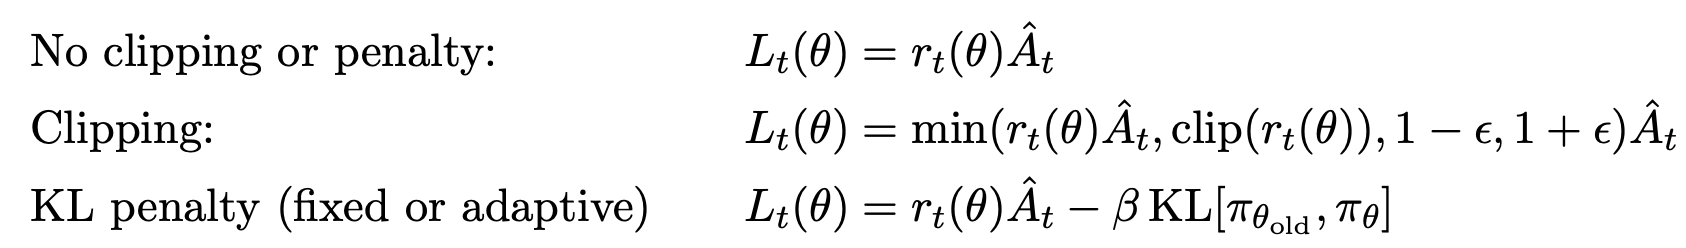
\includegraphics[width=\textwidth]{./imgs/loss.png}
  \end{figure}
  \vfill
\end{frame}

\begin{frame}
  \frametitle{As easy as 1, 2, 3}
  \vfill
  \begin{figure}[ht]
    \centering
    
\includegraphics[width=\textwidth]{./imgs/4.png}
    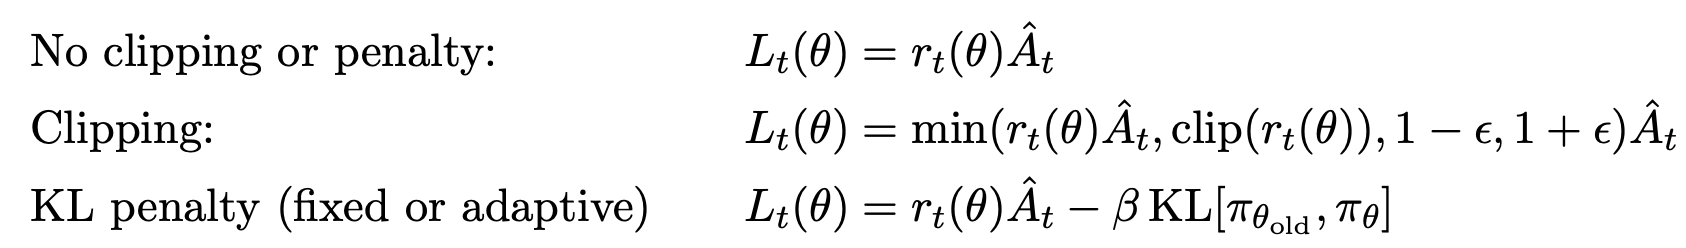
\includegraphics[width=\textwidth]{./imgs/loss.png}
  \end{figure}
  \vfill
  \begin{enumerate}
    \item What are the inputs?
    \item What are the outputs?
  \end{enumerate}
\end{frame}

\begin{frame}
  \frametitle{As easy as 1, 2, 3}
  \vfill
  \begin{figure}[ht]
    \centering
    
\includegraphics[width=\textwidth]{./imgs/4.png}
    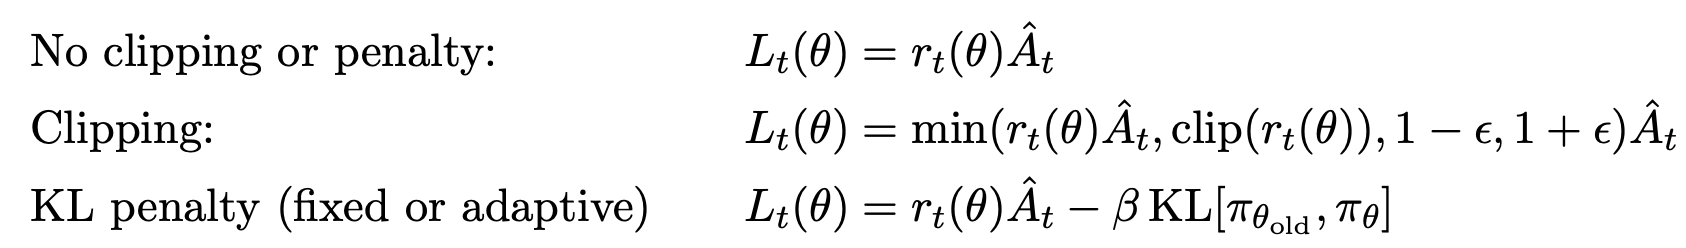
\includegraphics[width=\textwidth]{./imgs/loss.png}
  \end{figure}
  \vfill
  \begin{enumerate}
    \item What are the inputs? - $r_t(\theta) = \frac{\pi_\theta(a_t
      | s_t)}{\pi_{\theta_{old}}(a_t | s_t)}$, $\hat{A}_t$, $\epsilon$
    \item What are the outputs? - $L_t$!!!!!
  \end{enumerate}
\end{frame}

\section*{Pytorch}

\begin{frame}
  \frametitle{Pytorch}
  \begin{enumerate}
    \item Now we have a loss function $L_t$ that we want to minimize
      by changing model parameters $\theta$
      \vfill
    \item How do we do that?
  \end{enumerate}
\end{frame}

\begin{frame}
  \frametitle{Pytorch}
  \begin{enumerate}
    \item Now we have a loss function $L_t$ that we want to minimize
      by changing model parameters $\theta$
      \vfill
    \item How do we do that? - Gradient descent!
  \end{enumerate}
\end{frame}

\begin{frame}
  \frametitle{Simple Linear Regression Example}
  \vfill
  \begin{figure}[ht]
    \centering
    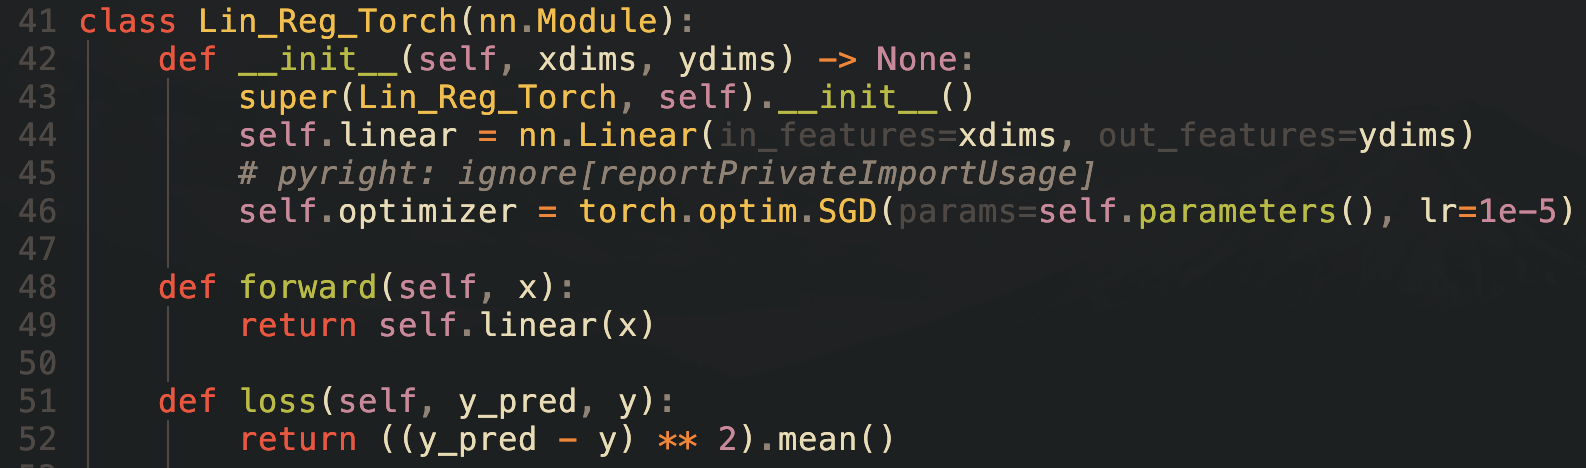
\includegraphics[width=\textwidth]{./imgs/pytorch_lin.png}
  \end{figure}
  \vfill
\end{frame}

\begin{frame}
  \frametitle{Simple Linear Regression Example}
  \begin{figure}[ht]
    \centering
    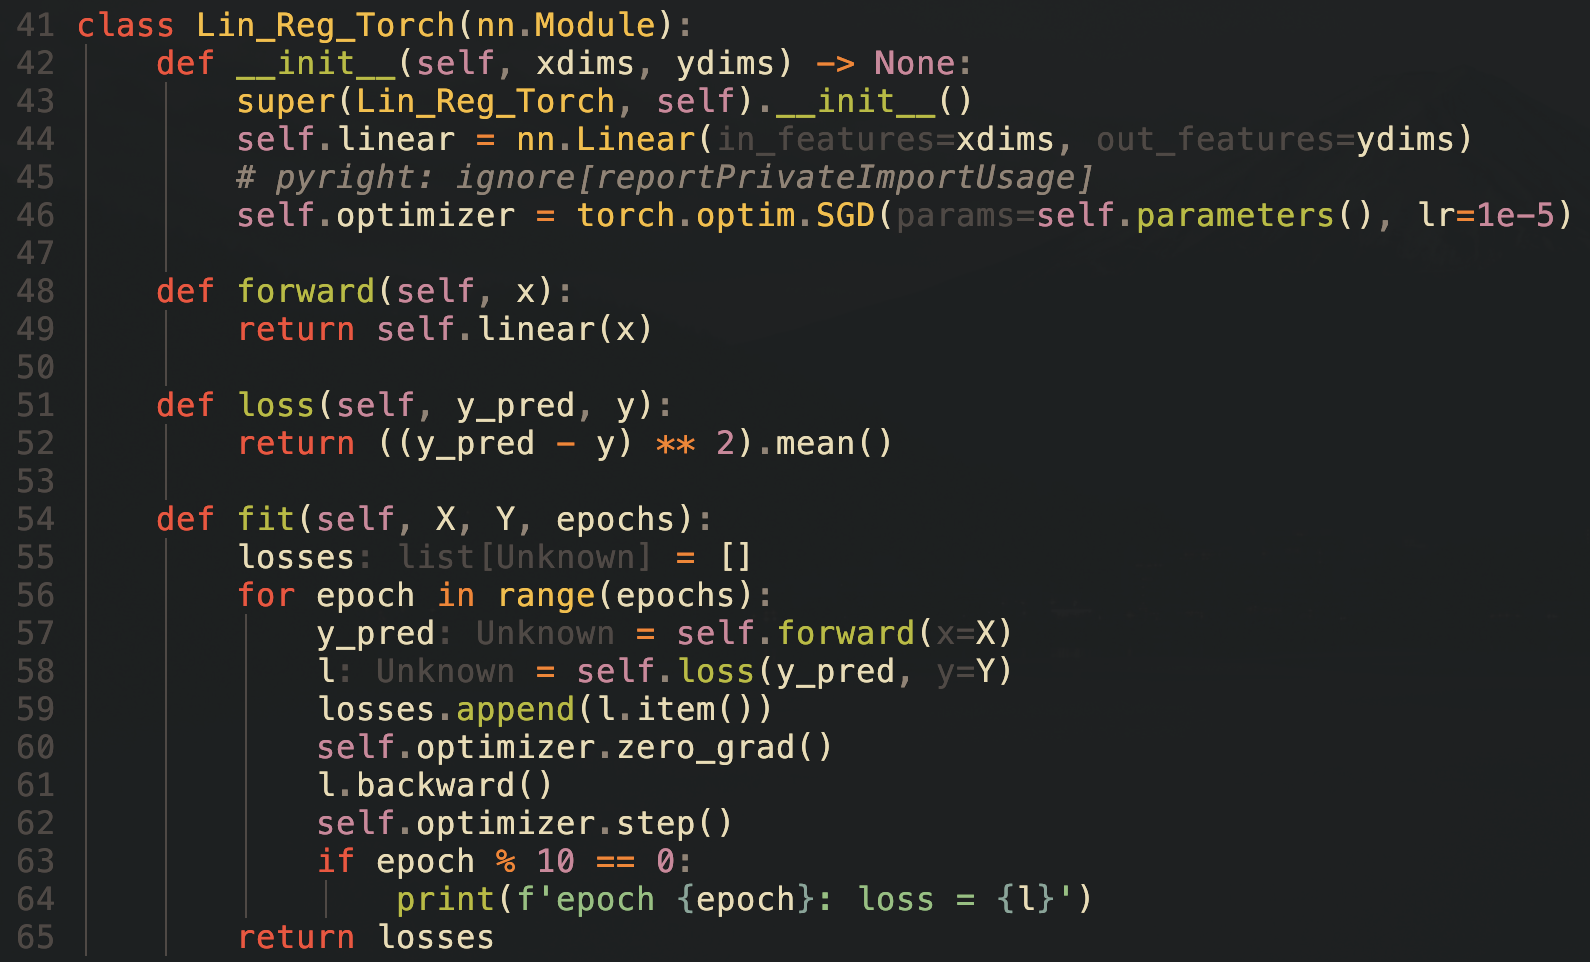
\includegraphics[width=\textwidth]{./imgs/pytorch_lin_fit.png}
  \end{figure}
\end{frame}

\begin{frame}
  \frametitle{PPO Pytorch}
  \begin{enumerate}
    \item PPO Assumes an Actor-Critic architecture
      \vfill
    \item One network for the policy $\pi_\theta$ and one for the
      value function $V^{\pi_\theta}$
  \end{enumerate}
\end{frame}

\begin{frame}
  \frametitle{PPO Pytorch}
  \begin{centering}
    \[
      \text{To the code!}
    \]
  \end{centering}
\end{frame}

\begin{frame}{Thank you!}
  Helpful Links
  \vfill
  \begin{enumerate}
    \item Up to data PPO paper - https://arxiv.org/abs/1707.06347
    \item Code - https://github.com/GersiD/ML/tree/main/RL/PPO
    \item Slides - Email me Gersi.Doko@unh.edu
  \end{enumerate}
\end{frame}

\end{document}
